\documentclass[11pt,a4paper]{article}

\usepackage[T1]{fontenc}
\usepackage[utf8]{inputenc}
\usepackage{lmodern}
\usepackage[margin=2.5cm]{geometry}
\usepackage{amsmath,amssymb}
\usepackage{graphicx}
\usepackage{booktabs}
\usepackage{array}
\usepackage[font=small,labelfont=bf]{caption}
\usepackage[authoryear,round]{natbib}
\usepackage{xcolor}
\usepackage{url}
% every link is black and has no frame. Only the web addresses in the reference list are meant to be followed.
\usepackage[hidelinks]{hyperref}
\setlength{\parskip}{0.4em}
\setlength{\parindent}{0pt}
\bibliographystyle{plainnat}
\newcolumntype{R}[1]{>{\raggedleft\arraybackslash}p{#1}}

% A work is named in the running text without brackets or years. Its full entry is in the reference list.
\newcommand{\mention}[1]{\citeauthor*{#1}}
\newcommand{\JT}{J_T}
\newcommand{\Jl}{J_\lambda}

\title{Zone-Based Local Search for Last-Mile Routing:\\
Large Neighbourhood Search and Simulated Annealing\\
Compared with OR-Tools on the Amazon Routing Challenge Data}

\author{Prof.\ Dhananjay Thiruvady\\Deakin University
\and Prof.\ Sutharshan Rajasegarar\\Deakin University
\and Lakshay Shrivastava\\Indian Institute of Technology Kharagpur}
\date{\today}

\begin{document}
\maketitle

\begin{abstract}
Last-mile delivery is the final step of a supply chain, in which a driver brings the parcels of one day from a depot to the customers' doors. For one driver this is a travelling salesman problem, but real drivers do not simply follow the shortest tour. They follow habits and local knowledge, and they tend to finish one neighbourhood before they start the next. We study how general-purpose local search copes with both aims, a short travel time and a route that resembles the one a driver would choose. We use the real routes of the 2021 Amazon Last Mile Routing Research Challenge and compare Google OR-Tools with large neighbourhood search on the whole route and with a zone-based pipeline. The pipeline first fixes the order of the delivery zones and then optimises windows of neighbouring zones, with large neighbourhood search or with simulated annealing inside each window. A single penalty for changing zones lets the same method move between short routes and tidy routes, and the zone order can be copied from earlier routes of the same depot. We measure travel time, zone changes and the challenge's own similarity score, and we state clearly what these measurements can and cannot show.
\end{abstract}

\section{Introduction}
Last-mile delivery is the last step of a supply chain. A van leaves a depot with the parcels of one day and a driver brings them to the customers. At the level of one driver, finding the quickest tour is a travelling salesman problem (TSP) with about 150 stops. This is small enough for exact solvers, yet the shortest tour is often not what the driver does. Drivers know the streets, they avoid some turns, and they finish a neighbourhood before they enter the next one. A planner that ignores this may produce routes that are short on paper but that drivers do not follow.

The 2021 Amazon Last Mile Routing Research Challenge released 6,112 real routes together with the order in which the drivers visited the stops, and asked for routes that resemble those of experienced drivers rather than for the shortest tours. In this report we ask a narrower question. \emph{Given only the travel-time matrix and the zone label of each stop, how do general-purpose local-search methods compare with OR-Tools, both on travel time and on how much the routes look like the drivers' routes, and what does a zone-based decomposition change?} We do not try to reproduce the competition entry and we do not claim a new state of the art. Figure~\ref{fig:routes} shows the idea on one route.

\begin{figure}[t]
\centering
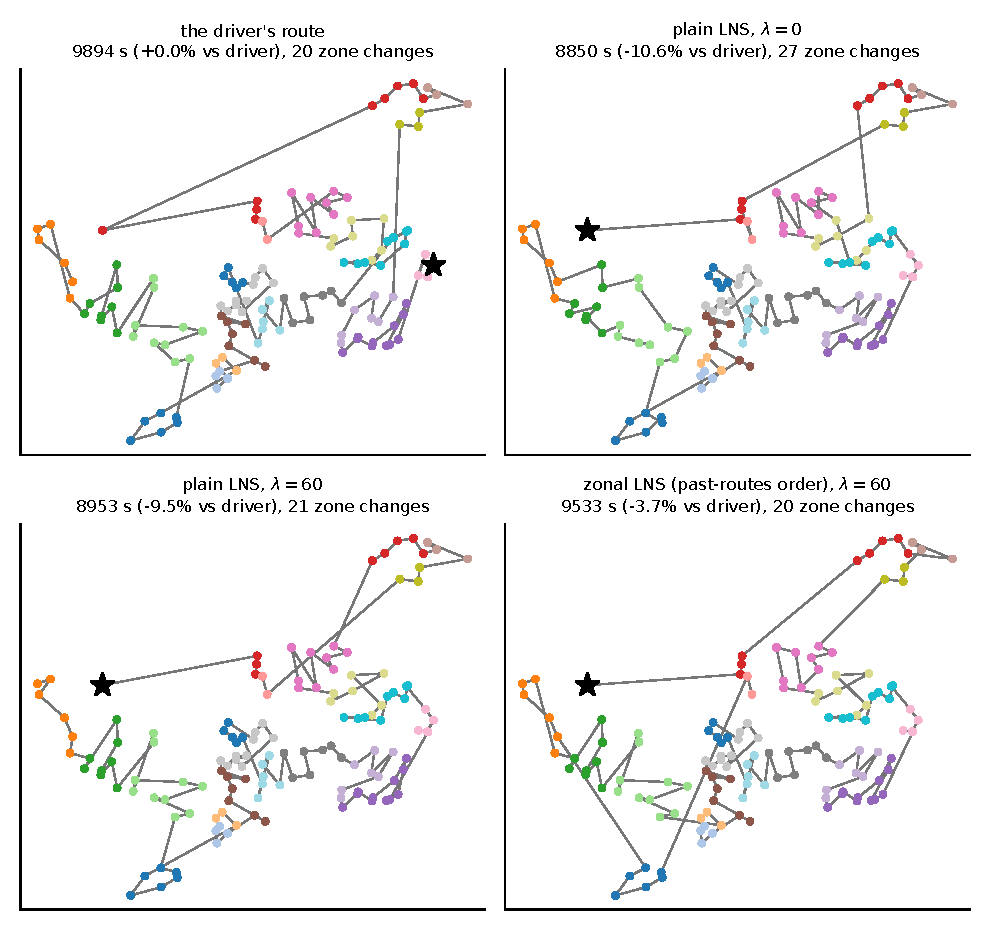
\includegraphics[width=0.78\linewidth]{figures/fig_routes}
\caption{One development route (137 stops, 21 zones, a high-quality route of median size), coloured by zone. The star marks the first stop and the depot lies outside the drawing. The shortest tours hop between zones more often than the driver. The zonal route follows the zone order of an earlier route and has about as many zone changes as the driver. This is a single example chosen by size, not a typical or best case. On this route the zonal route saves less travel time than the average zonal route in Table~\ref{tab:main}.}\label{fig:routes}
\end{figure}

\subsection{Contributions}
\begin{itemize}
  \item A comparison of three approaches with an OR-Tools baseline under one objective and one protocol. The approaches are plain LNS, zonal LNS and zonal SA (Section~\ref{sec:methods}). The third tests simulated annealing inside the zone pipeline.
  \item A zone-change penalty $\lambda$ that lets one method trade travel time against tidiness (Section~\ref{sec:lambda}).
  \item A final evaluation on the 3,052 routes of the challenge's separate evaluation folder, with several random seeds and paired comparisons (Section~\ref{sec:main}), and a study of the zonal pipeline on development routes (Section~\ref{sec:dev}).
\end{itemize}

\subsection{Structure of this report}
Section~\ref{sec:related} reviews the papers we studied and the classical methods we build on. Section~\ref{sec:data} describes the data and Section~\ref{sec:problem} defines the problem and the metrics, including $\lambda$. Section~\ref{sec:methods} describes the methods and Section~\ref{sec:setup} says which data each method uses and how it was tuned. Results are in Section~\ref{sec:results}. Section~\ref{sec:limits} discusses what they do and do not show and Section~\ref{sec:conclusion} concludes. Appendix~\ref{app:exact} checks LNS against exact solvers.

\section{Related work}\label{sec:related}
\paragraph{Challenge and winning solution.}
The challenge data are described by \mention{merchan2022}, the technical reports of the participants are collected by \mention{winkenbach2021}, and the rules and data are hosted by \mention{challengeweb}. The winning team, \mention{cook2022}, extend the Lin--Kernighan heuristic of \mention{linkernighan1973} as implemented by \mention{helsgaun2000} and extended to constrained problems by \mention{helsgaun2017}. They add penalties for visiting zones in an order that earlier drivers did not use, learn this order from ``reference routes'' of the same depot, and add penalties for leaving clusters of zones that share part of their zone ID. We use two of their ideas, the zone-change penalty and the reference-route zone order, with simpler optimisers of our own.

\paragraph{Learning-based approaches.}
\mention{ruizfas} train a graph neural network encoder with a pointer-network decoder per geographical zone on the Los Angeles routes of the challenge. \mention{kool2019} propose an attention model trained with reinforcement learning for TSP and vehicle-routing variants on random instances of up to 100 nodes. \mention{ozarik} frame the challenge as an inverse-optimisation problem, generate a pool of candidate sequences and select among them with a regression model that predicts the challenge score. \mention{xu2026} study order dispatching and routing for last-mile \emph{pickup} with deep reinforcement learning, which is a different problem from ours but uses graph attention for routing in a last-mile setting. During this project we also trained a zone-order graph neural network. It gave no gain over copying a reference route and is not part of the methods compared here.

\paragraph{Local search and OR-Tools.}
Large neighbourhood search was introduced by \mention{shaw1998} and made adaptive by \mention{ropke2006}. It repeatedly removes a set of stops from a solution and reinserts them. Simulated annealing, introduced by \mention{kirkpatrick1983}, accepts a worsening move with a probability that decreases over time. Our simulated annealing uses the 2-opt move of \mention{croes1958} and two further moves. The routing solver of the OR-Tools library, maintained by \mention{ortools}, is our baseline.

\section{Amazon routing data}\label{sec:data}
The challenge has a training folder with 6,112 routes from 17 depots (``stations'') in the United States and a separate evaluation folder with 3,052 routes from 18 depots. Each route is the day of one driver. For each route the data give the latitude and longitude of the stops, a zone ID for each stop, the estimated travel time in seconds between every pair of stops, package information, and the order in which the real driver visited the stops. Amazon rated each driver route in the training folder as high, medium or low quality (2,718, 3,292 and 102 routes). Table~\ref{tab:data} gives the numbers we computed from the files and Figure~\ref{fig:data} shows the distributions for the training folder.

\begin{table}[t]
\centering\small
\caption{The data as we use them (numbers computed from the files). The development routes are a random sample of the training folder, see Section~\ref{sec:setup}.}\label{tab:data}
\begin{tabular}{lrr}
\toprule
 & Training folder & Evaluation folder \\
\midrule
Routes & 6,112 & 3,052 \\
Depots (stations) & 17 & 18 \\
Stops per route, mean (min--max) & 147.0 (32--237) & 140.9 (18--224) \\
Zones per route, mean (min--max) & 20.0 (4--47) & 19.4 (5--47) \\
Driver quality: high / medium / low & 2,718 / 3,292 / 102 & not given \\
Zone changes of the drivers, mean & 20.3 on the development routes & 19.8 \\
\bottomrule
\end{tabular}
\end{table}

\begin{figure}[t]
\centering
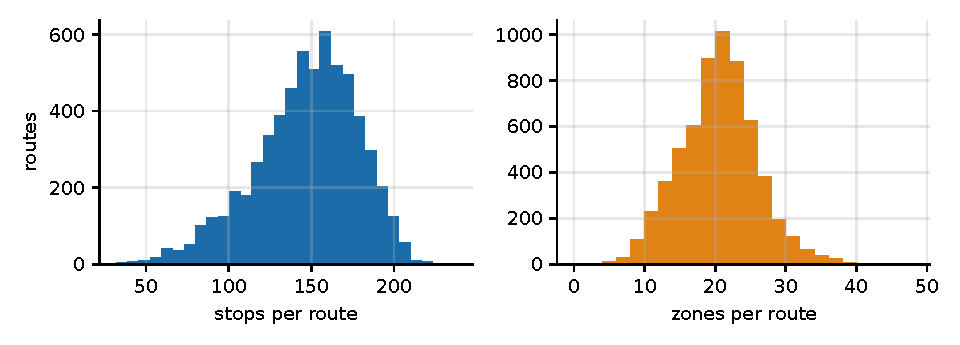
\includegraphics[width=0.8\linewidth]{figures/fig_data}
\caption{Size of the routes in the 6,112 training routes: stops per route (left) and zones per route (right).}\label{fig:data}
\end{figure}

\paragraph{Travel times are asymmetric.} The time from stop $i$ to stop $j$ is generally not the same as from $j$ to $i$ because of one-way streets and traffic, so each route is an \emph{asymmetric} TSP. The times are estimates supplied with the data and not measured values.

\paragraph{Zones.} Each stop carries a zone ID such as \texttt{A-2.1E}, set by Amazon's own planning. Drivers tend to finish a zone before they enter the next one, which is why zones matter. A short tour that jumps between zones is often not what a driver would do. About 0.7\% of the stops of the training folder (in 42\% of its routes) have no zone ID, and we give each of them the zone of the nearest stop of the same route (Euclidean distance on latitude and longitude). After this step no stop of the evaluation folder is without a zone.

\paragraph{What we do not use.} The data also contain delivery time windows, package sizes and service times. We do not use them. Our objective is travel time, so our routes are not checked against these constraints (Section~\ref{sec:limits}).

\section{Problem and metrics}\label{sec:problem}
\subsection{The routing problem}
A route has a depot $0$ and $n$ delivery stops $1,\dots,n$ (about 141 to 147 on average). $T_{ij}$ is the estimated travel time from $i$ to $j$ in seconds and $z(i)$ is the zone of stop $i$. A solution is an order $\pi=(\pi_0=0,\pi_1,\dots,\pi_n)$ of all stops, starting at the depot. Following the challenge, the route is an open path, so we do not add the way back to the depot. Its travel time is
\begin{equation}
\JT(\pi)=\sum_{k=0}^{n-1} T_{\pi_k\pi_{k+1}} .
\end{equation}
Unless stated otherwise, ``travel time'' means this quantity. We always report it relative to the driver's own route $\pi^d$ on the same route, $\JT(\pi)/\JT(\pi^d)-1$, in percent. A value of $-10\%$ means 10\% less estimated travel time than the driver.

\subsection{Zone changes and the penalty $\lambda$}
The number of \emph{zone changes} of a route is the number of consecutive stops that belong to different zones,
\begin{equation}
S(\pi)=\sum_{k=1}^{n-1}\mathbf 1\!\left[z(\pi_k)\neq z(\pi_{k+1})\right].
\end{equation}
A route that visits each zone in one block has $S=Z-1$ for $Z$ zones. The real drivers average 19.8 zone changes on the evaluation routes, with about 19 zones. A short tour that hops between zones has many more.

The parameter $\lambda\ge 0$ (seconds) is a \emph{price for a zone change}. The methods minimise
\begin{equation}
\Jl(\pi)=\JT(\pi)+\lambda\bigl(S(\pi)+1\bigr)
=\sum_{k=0}^{n-1} C_{\pi_k\pi_{k+1}},\qquad C_{ij}=T_{ij}+\lambda\,\mathbf 1\!\left[z(i)\neq z(j)\right],
\end{equation}
so a route that leaves a zone must save at least $\lambda$ seconds of driving to be preferred. (The $+1$ is the unavoidable first step from the depot and changes nothing.) With $\lambda=0$ the methods look only at travel time. Larger values give tidier routes with fewer zone changes, at some cost in travel time. The penalty is only used inside the optimisers, and all reported times are real estimated travel times without penalties. We report $\lambda=0$ and $\lambda=60$ s. We chose $\lambda=60$ s as a moderate setting because it brings the number of zone changes close to the drivers' number on the development routes (Section~\ref{sec:lambda}). It is a fixed choice and not an optimised one.

\subsection{The official challenge score}
The challenge scores a proposed sequence $B$ against the driver's sequence $A$ by how similar they are. \emph{Lower is better and the driver's own sequence scores 0}. The score is the product $\mathrm{SD}\times\mathrm{ERP}_{\mathrm{norm}}$ of two quantities.
\begin{itemize}
\item $\mathrm{SD}$ (sequence deviation) measures how far consecutive stops of $B$ are apart in $A$:
$\mathrm{SD}(A,B)=\frac{2}{n(n-1)}\sum_{k}\bigl(|\mathrm{pos}_A(B_{k+1})-\mathrm{pos}_A(B_k)|-1\bigr)$, where $\mathrm{pos}_A(x)$ is the position of stop $x$ in $A$. It is 0 if $B$ visits the stops in the same order as $A$.
\item $\mathrm{ERP}_{\mathrm{norm}}$ is an edit distance (edit distance with real penalty) between the two sequences. Replacing one stop by another costs their travel time (scaled by the standard deviation of the travel-time matrix), inserting or deleting a stop costs 1000, and the total is divided by the number of edit operations.
\end{itemize}
We re-implemented this score from the public scoring code of the challenge. We checked it on simple cases (the driver's own sequence scores 0, and random orders score about 0.9) but could not compare it with Amazon's own scorer on the same submissions, so small differences are possible. The score is only a \emph{proxy} for ``looks like what the driver did''. It does not tell us whether a driver would accept the route.

\subsection{Comparing methods}
All methods are run on the same routes. For two methods $a$ and $b$ we compute the difference of their results route by route and report its mean, a 95\% interval (mean $\pm\,1.96$ standard errors over routes) and the share of routes on which $a$ is better. If the interval excludes zero we treat the difference as real. These intervals describe variation between routes only. Variation between random seeds is shown separately.

\section{Methods}\label{sec:methods}
We compare a baseline and three approaches. Every method gets the same input (the matrix $T$ and the zones) and minimises the same objective $\Jl$. The starting route of LNS and SA is the nearest-neighbour route under $C$.

\subsection{Baseline: OR-Tools}\label{sec:ortools}
We use the OR-Tools routing solver (version 9.15) with one vehicle that starts at the depot and ends at an added dummy node whose arcs cost zero. This turns the open path into the closed route the solver expects. Costs are the matrix $C$ multiplied by 10 and rounded to integers, because the solver needs integer costs. The first solution is built by the strategy \texttt{PATH\_CHEAPEST\_ARC} (always take the cheapest next arc). It is then improved by \emph{guided local search} for a fixed wall-clock time of 10 s per route. All other settings are the defaults and we did not tune them. Because the search is limited by time, its result depends slightly on the load of the machine. On the development routes two runs gave $-10.82\%$ and $-10.38\%$ travel time. OR-Tools has no training and uses no historical data.

\subsection{Plain LNS}\label{sec:lns}
Large neighbourhood search keeps a current route and, in each iteration, (i) removes a group of $k$ stops (``destroy''), (ii) puts them back at the cheapest positions (``repair''), and (iii) accepts or rejects the new route. Our implementation (compiled with Numba for speed) works as follows.
\begin{itemize}
\item \textbf{Destroy.} One of four rules is chosen at random with adaptive probabilities. The rules remove $k$ random stops, or the $k$ stops most related to a random stop (smallest travel time to it), or the $k$ stops that cause the largest detour, or stops of one zone. The size $k$ is drawn at random between $\max(2,\lfloor m/40\rfloor)$ and $\max(3,\lfloor m/2\rfloor)$ for $m$ movable stops, so up to \emph{half} of the route can be removed at once. This upper limit was the only LNS setting that mattered on validation routes. A limit of $m/8$ was 1.4 points worse at equal run time.
\item \textbf{Repair.} Either \emph{greedy} insertion (repeatedly insert the stop and position with the smallest cost increase) or \emph{regret-2} insertion (insert the stop that would lose most if it did not get its best position).
\item \textbf{Acceptance.} A simulated-annealing rule. A better route is accepted, and a worse one is accepted with probability $\exp(-\Delta/\tau)$. The temperature $\tau$ starts at $0.02\,\Jl/n$ and decreases geometrically to $0.01$. The best route found is returned.
\item \textbf{Operator weights.} The probability of each destroy and repair rule is updated from how well it did, in the adaptive scheme reviewed in Section~\ref{sec:related}.
\item \textbf{Budget.} 5,000 iterations, which takes about 2 s per route.
\end{itemize}

\subsection{Zonal methods: zone order, then overlapping windows}\label{sec:zonal}
The zonal pipeline (Figure~\ref{fig:pipeline}) splits the route into zones and uses the zone structure of the drivers' routes. It has three steps.

\begin{figure}[t]
\centering
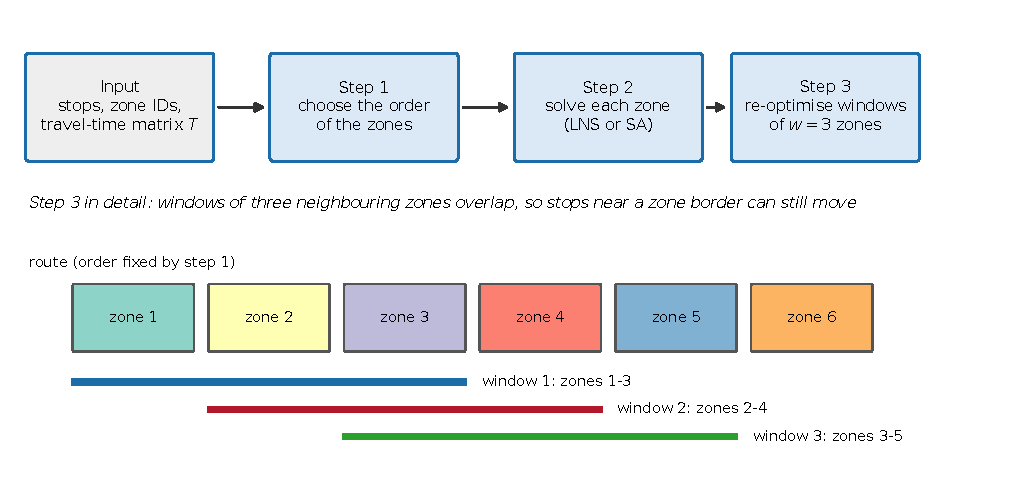
\includegraphics[width=0.95\linewidth]{figures/fig_pipeline}
\caption{The zonal pipeline. Windows of $w=3$ neighbouring zones overlap, so a stop close to a zone border can still move into the neighbouring zone's part of the route when the window is re-optimised.}\label{fig:pipeline}
\end{figure}

\paragraph{Step 1: zone order.} We choose the order in which the zones are visited. We use two ways to do this.
\begin{itemize}
\item \emph{Order by zone routing.} Treat every zone as one node, with the average travel time between the stops of two zones as the distance, and solve this small routing problem (about 20 nodes) with the LNS of Section~\ref{sec:lns}. This uses no historical data.
\item \emph{Order from past routes.} For a new route we look up the earlier routes of the same depot and take the one that shares the most zones with it, weighting routes by the driver's quality rating (high 2, medium 1.5, low 1). The zones of the new route are visited in the order in which that earlier driver first entered them. Zones the earlier route never visited are inserted at the cheapest place. This is the reference-route idea of the winning team (Section~\ref{sec:related}) in a simplified form. It needs earlier routes of the same depot, and it copies driver behaviour, so a better official score is partly expected.
\end{itemize}

\paragraph{Step 2: solve each zone.} In the chosen order, each zone is solved as a small path that starts where the previous zone ended. The result is a route in which every zone forms one block.

\paragraph{Step 3: overlapping windows.} A window of $w=3$ consecutive zones is re-optimised with the stop before the window and the stop after it kept fixed, and then the window slides by one zone. Consecutive windows overlap in two zones, which lets stops near a border move. The objective $\Jl$ is the same as before, so with $\lambda>0$ a stop only moves to another zone if it saves more than $\lambda$ seconds. The zone order fixes the coarse structure of the route, so its quality limits what the windows can achieve.

\subsection{Zonal LNS and zonal SA}\label{sec:sa}
In \emph{zonal LNS} the optimiser inside each zone and each window is the LNS of Section~\ref{sec:lns}, with 1,000 iterations per zone and 1,500 per window. In \emph{zonal SA} it is simulated annealing. Each iteration proposes one move, which is a 2-opt reversal of a segment (probability 0.4), a relocation of a segment of one to three stops (0.4) or a swap of two stops (0.2). The move is accepted if it is better, or with probability $\exp(-\Delta/\tau)$ otherwise. The temperature falls geometrically from $\tau_0=0.5\,\Jl/n$ to $0.001$. Because the matrix is asymmetric, reversing a segment changes its cost, and our 2-opt evaluation accounts for it. We use 50,000 iterations per zone and 300,000 per window. Each SA iteration is much cheaper than an LNS iteration. The starting temperature was chosen on validation routes with SA on whole routes, where hotter starts were clearly better than $0.05$, and the same value was used for zonal SA. Table~\ref{tab:methods} summarises the four methods.

\begin{table}[t]
\centering\small
\caption{The baseline and the three approaches with their settings.}\label{tab:methods}
\begin{tabular}{p{3.0cm}p{4.2cm}p{4.2cm}p{2.6cm}}
\toprule
Method & Search & Settings & Uses past routes? \\
\midrule
OR-Tools (baseline) & guided local search & 10 s per route, default settings & no \\
Plain LNS & destroy and repair on the whole route & 5,000 iterations, up to $m/2$ stops removed & no \\
Zonal LNS & zone order, zones, windows with LNS & $w=3$, 1,000 + 1,500 iterations & only with the past-routes order \\
Zonal SA & as zonal LNS with SA inside & $w=3$, 50,000 + 300,000 iterations & only with the past-routes order \\
\bottomrule
\end{tabular}
\end{table}

\section{Experimental setup}\label{sec:setup}
Figure~\ref{fig:design} shows which routes are used for which purpose.

\begin{figure}[t]
\centering
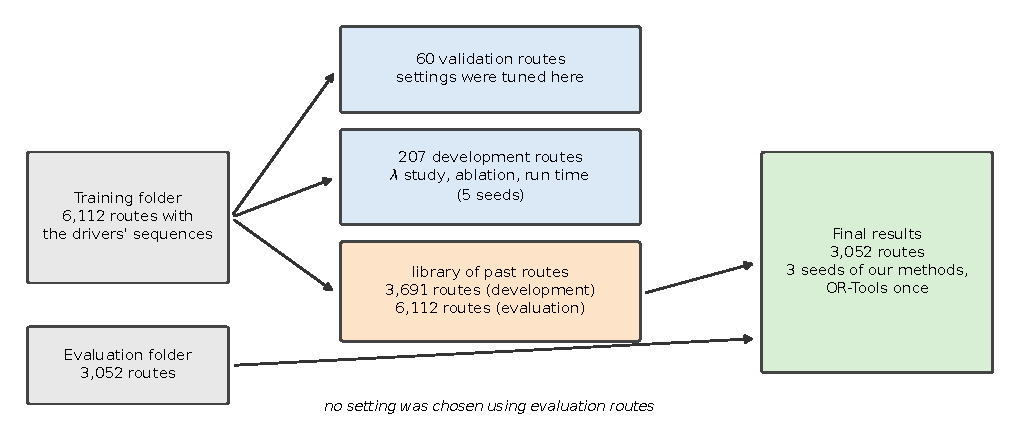
\includegraphics[width=0.95\linewidth]{figures/fig_design}
\caption{Which routes are used for what. Settings were tuned on 60 validation routes. The development routes were used for the $\lambda$ study, the ablation and the run times. The 3,052 evaluation routes were used only for the final results.}\label{fig:design}
\end{figure}

\paragraph{Data splits.} Each training route is assigned to a training, validation or test part by a hash of its route ID (60\%, 20\%, 20\%). The assignment never changes and no route is in two parts. Because the methods are compute-heavy, we first worked with a random sample of 1,000 of the 6,112 routes (drawn once with a fixed seed). Its test part has \textbf{207 routes} (148 stops and 20 zones on average, 16 depots), which we call the \emph{development routes}. The $\lambda$ study, the ablation and the run times of Section~\ref{sec:dev} use them, and so does the choice of $\lambda=60$ s. The 3,052 routes of the \emph{evaluation folder} were not used for any choice. A pilot run on 300 of them only checked that the code worked, and no setting was changed afterwards. The final results of Section~\ref{sec:main} use all of them.

\paragraph{What each method uses.} Only one component learns from data, the zone order from past routes. Its library of past routes is made of the 3,691 training routes of the hash split for the development routes and of all 6,112 training-folder routes for the evaluation routes. A route is never its own reference, and no evaluation route is in the training folder. Of the 3,052 evaluation routes, 3,051 come from a depot that has routes in the library. One route comes from a depot without any (DBO6), and for this route the zones are ordered only by the cheapest-insertion rule. Nothing else is trained. The remaining settings (iteration counts, neighbourhood size, SA temperature, window width) were chosen by trying alternatives on 60 \emph{validation} routes. The zonal settings were chosen before we fixed the missing zone IDs and were not re-tuned afterwards. The two values of $\lambda$ are a fixed choice. OR-Tools uses default settings and no data.

\paragraph{Seeds.} The random choices of LNS, SA and the zonal methods are controlled by a seed. Our methods were run with seeds 0 to 2 (three runs) on the evaluation routes and with seeds 0 to 4 (five runs) on the development routes. The tables report the mean over seeds of the average over routes, and the standard deviation of that mean over the seeds. OR-Tools is limited by time rather than by a seed, so it appears as one run. The paired comparisons use seed~0.

\paragraph{Implementation and timing.} Code is written in Python (3.14) with NumPy and Numba (0.68), and OR-Tools is version 9.15. The evaluation was run with 10 parallel processes on a Windows PC with a 14-core processor. One seed of all eleven settings took 34 to 44 minutes and OR-Tools took 107 minutes. Because the processes share the machine, the evaluation runs give no clean run times, and OR-Tools, which is limited by time, may be slightly affected. Run times in Section~\ref{sec:dev} come from a separate clean run on 20 development routes, in one process with nothing else running. Absolute times depend on the machine, so the ratios matter more.

\section{Results}\label{sec:results}
\subsection{Main comparison on the evaluation routes}\label{sec:main}
Table~\ref{tab:main} shows the baseline and the three approaches on the 3,052 evaluation routes at $\lambda=0$ (travel time only) and $\lambda=60$ s. Figure~\ref{fig:tradeoff} shows the same results as a trade-off between travel time and similarity to the driver.

\begin{table}[t]
\centering\small
\caption{Results on the 3,052 evaluation routes, seeds 0 to 2 (mean $\pm$ standard deviation over seeds, OR-Tools one run). Travel time is relative to the driver's route (negative means less). The driver has 19.8 zone changes and official score 0 by definition. ``Order by zone routing'' and ``order from past routes'' are the two ways to choose the zone order (Section~\ref{sec:zonal}).}\label{tab:main}
\begin{tabular}{lR{3.1cm}R{2.4cm}R{2.9cm}}
\toprule
Method & Travel time vs.\ driver (\%) & Zone changes & Official score \\
\midrule
\multicolumn{4}{l}{\textit{$\lambda=0$ (travel time only)}}\\
OR-Tools (10 s) & $-10.96$ & $35.7$ & $0.0858$ \\
plain LNS & $-13.91\pm0.01$ & $33.4\pm0.0$ & $0.0770\pm0.0001$ \\
zonal LNS, order by zone routing & $-11.12\pm0.04$ & $29.4\pm0.0$ & $0.0655\pm0.0002$ \\
zonal LNS, order from past routes & $-9.09\pm0.00$ & $29.1\pm0.0$ & $0.0499\pm0.0001$ \\
zonal SA, order by zone routing & $-11.13\pm0.04$ & $29.7\pm0.1$ & $0.0664\pm0.0003$ \\
zonal SA, order from past routes & $-9.13\pm0.00$ & $29.4\pm0.0$ & $0.0508\pm0.0001$ \\
\midrule
\multicolumn{4}{l}{\textit{$\lambda=60$ s (balanced)}}\\
OR-Tools (10 s) & $-9.48$ & $21.2$ & $0.0594$ \\
plain LNS & $-11.48\pm0.01$ & $20.4\pm0.0$ & $0.0531\pm0.0001$ \\
zonal LNS, order by zone routing & $-9.21\pm0.03$ & $19.5\pm0.0$ & $0.0501\pm0.0002$ \\
zonal LNS, order from past routes & $-7.22\pm0.01$ & $19.5\pm0.0$ & $0.0384\pm0.0001$ \\
zonal SA, order by zone routing & $-9.35\pm0.02$ & $19.6\pm0.0$ & $0.0506\pm0.0003$ \\
zonal SA, order from past routes & $-7.41\pm0.01$ & $19.6\pm0.0$ & $0.0391\pm0.0001$ \\
\bottomrule
\end{tabular}

\end{table}

\begin{figure}[t]
\centering
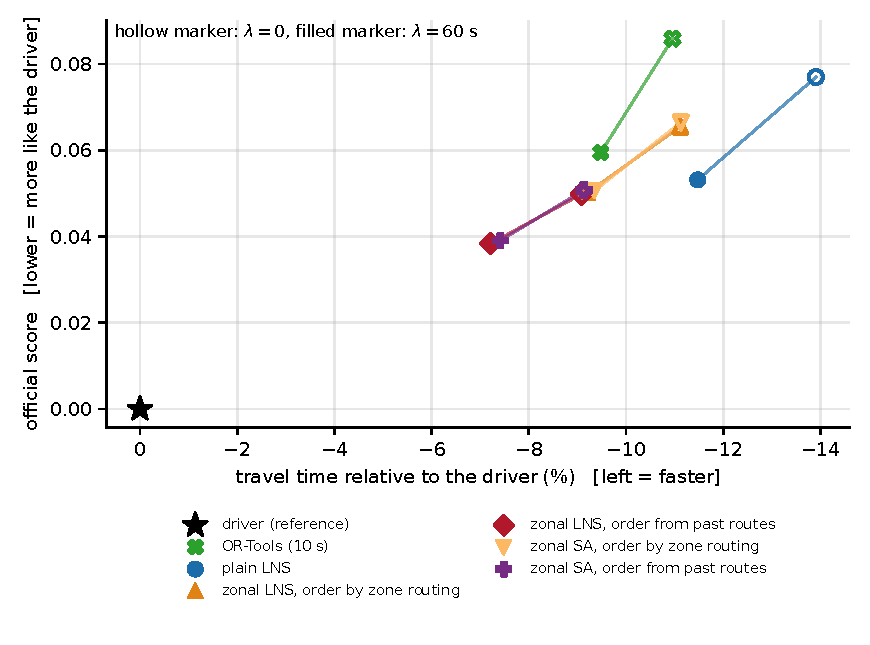
\includegraphics[width=0.78\linewidth]{figures/fig_eval_tradeoff}
\caption{Travel time against official score on the evaluation routes. Each method appears twice, joined by a line, with a hollow marker for $\lambda=0$ and a filled marker for $\lambda=60$ s. Points further left save more travel time and points lower down are more like the driver. The spread over seeds is too small to show.}\label{fig:tradeoff}
\end{figure}

We observe the following.
\begin{enumerate}
\item \textbf{Plain LNS finds the shortest routes.} At $\lambda=0$ it saves 13.9\% of estimated travel time against the drivers and OR-Tools at 10 s saves 11.0\%. At $\lambda=60$ s the figures are 11.5\% and 9.5\%.
\item \textbf{Shorter does not mean more like the driver.} Plain LNS has 33.4 zone changes per route at $\lambda=0$ against the drivers' 19.8, and its official score is 0.077. OR-Tools has 35.7 changes and a score of 0.086.
\item \textbf{Zonal methods give tidier routes.} They cut the zone changes to between 29.1 and 29.7 at $\lambda=0$ and to 19.5 or 19.6 at $\lambda=60$, which is the drivers' level. They give up travel time compared with plain LNS (11.1\% at $\lambda=0$ and 9.2\% at $\lambda=60$ with the zone-routing order).
\item \textbf{The zone order from past routes has the largest effect on the official score.} With it, zonal LNS reaches 0.050 at $\lambda=0$ and 0.038 at $\lambda=60$. With the zone-routing order the scores are 0.066 and 0.050, and for plain LNS they are 0.077 and 0.053. The price is about 2 points of travel time (9.1\% and 7.2\% saved).
\item \textbf{Zonal SA and zonal LNS give nearly the same routes.} Their travel times differ by at most 0.20 points and their official scores by at most 0.0009. At $\lambda=60$ with the past-routes order SA saves a little more travel time ($0.19\pm0.03$ points, Table~\ref{tab:paired}) and needs about five times as long (Section~\ref{sec:dev}).
\item \textbf{The seeds hardly matter.} Over three seeds the standard deviation of the average travel time is at most 0.04 points and that of the official score at most 0.0003. This is far smaller than the differences between methods.
\end{enumerate}

\subsection{Paired comparisons}\label{sec:paired}
Table~\ref{tab:paired} gives the route-by-route differences between selected pairs of methods (seed~0). Negative values mean that the first method is better. At $\lambda=0$, plain LNS beats OR-Tools by $2.96\pm0.07$ points of the driver's travel time and is better on 97\% of the routes. Zonal LNS with the zone-routing order is about level with OR-Tools ($0.21\pm0.10$ points better, better on 57\% of the routes) and loses to plain LNS by $2.75\pm0.09$ points. At $\lambda=60$, zonal LNS with the past-routes order saves $2.26\pm0.14$ points less travel time than OR-Tools but has a lower official score by $0.0210\pm0.0011$, on 79\% of the routes. Averaged over the seeds, this zonal route has more travel time than the driver on 5.9\% of the routes, against 0.07\% for plain LNS and 0.9\% for OR-Tools.

\begin{table}[t]
\centering\small
\caption{Paired differences on the evaluation routes, seed 0 (first method minus second, negative means the first method is better). The last column is the share of routes on which the first method is better.}\label{tab:paired}
\begin{tabular}{p{8.6cm}R{2.0cm}R{2.2cm}R{2.0cm}}
\toprule
Comparison & Difference & 95\% interval & First better \\
\midrule
\multicolumn{4}{l}{\textit{travel time (points)}}\\
$\lambda=0$: plain LNS vs OR-Tools & $-2.96$ & $\pm0.07$ & 97\% \\
$\lambda=0$: zonal LNS (zone-routing order) vs OR-Tools & $-0.21$ & $\pm0.10$ & 57\% \\
$\lambda=0$: zonal LNS (zone-routing order) vs plain LNS & $+2.75$ & $\pm0.09$ & 7\% \\
$\lambda=0$: zonal SA vs zonal LNS (zone-routing order) & $+0.01$ & $\pm0.02$ & 49\% \\
$\lambda=60$: zonal SA vs zonal LNS (past-routes order) & $-0.19$ & $\pm0.03$ & 52\% \\
$\lambda=60$: plain LNS vs OR-Tools & $-2.01$ & $\pm0.06$ & 89\% \\
$\lambda=60$: zonal LNS (past-routes order) vs OR-Tools & $+2.26$ & $\pm0.14$ & 31\% \\
$\lambda=60$: zonal LNS (past-routes order) vs plain LNS & $+4.27$ & $\pm0.13$ & 5\% \\
\midrule
\multicolumn{4}{l}{\textit{official score}}\\
$\lambda=60$: zonal LNS (past-routes order) vs OR-Tools & $-0.0210$ & $\pm0.0011$ & 79\% \\
$\lambda=60$: zonal LNS (past-routes order) vs plain LNS & $-0.0147$ & $\pm0.0011$ & 72\% \\
$\lambda=60$: zonal LNS, past-routes vs zone-routing order & $-0.0115$ & $\pm0.0010$ & 66\% \\
\bottomrule
\end{tabular}

\end{table}

\subsection{By depot and by route size}\label{sec:depot}
Figure~\ref{fig:depot} shows $\lambda=60$ s for each depot with at least ten routes. The ranking of the methods is the same at all 17 depots. Plain LNS saves the most travel time, then OR-Tools, then the zonal method, and the zonal method with the past-routes order has the lowest official score. Between depots the saving of plain LNS ranges from 8.9\% to 17.8\% and that of the zonal method from 5.1\% to 12.5\%, so the differences between depots are larger than the differences between the methods. The official score of the zonal method ranges from 0.021 to 0.073. Figure~\ref{fig:dist} shows that the zonal method moves the whole distribution of route scores towards zero (40\% of its routes score below 0.02, against 14\% for plain LNS and 11\% for OR-Tools). The savings in travel time are largest on the shortest routes. For plain LNS they fall from 13.6\% on routes with up to 107 stops to between 10.5\% and 11.9\% on longer routes, and the zonal method stays about 4 to 5 points behind.

\begin{figure}[t]
\centering
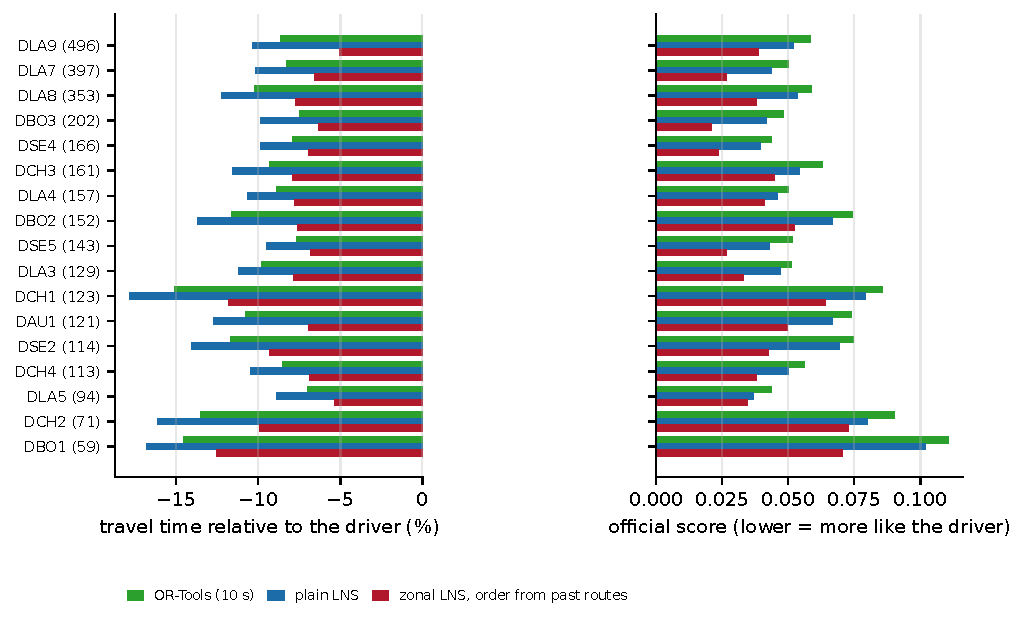
\includegraphics[width=0.95\linewidth]{figures/fig_eval_depot}
\caption{Results by depot at $\lambda=60$ s on the evaluation routes (mean over three seeds, the number of routes is in brackets). Left, travel time relative to the driver. Right, official score. Depot DBO6 has one route and is not shown.}\label{fig:depot}
\end{figure}

\begin{figure}[t]
\centering
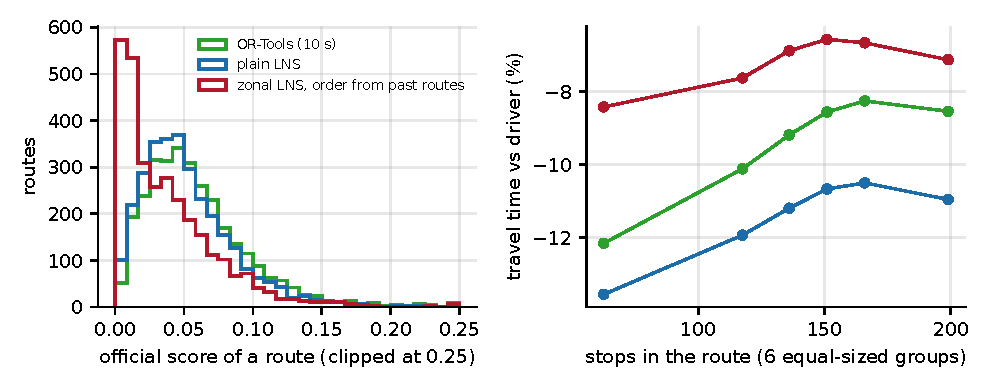
\includegraphics[width=0.95\linewidth]{figures/fig_eval_dist}
\caption{Spread over the evaluation routes at $\lambda=60$ s. Left, histogram of the official score of a route. Right, mean travel time relative to the driver by route size, using six groups of about 500 routes each (the colours are as in the left panel).}\label{fig:dist}
\end{figure}

\subsection{Studies on the development routes}\label{sec:dev}
The studies in Figure~\ref{fig:dev} and Table~\ref{tab:ablation} use the 207 development routes with seeds 0 to 4. The same methods on these routes give results close to the evaluation routes (Table~\ref{tab:main-dev}). For every method the travel time differs by at most 0.9 points and the official score by at most 0.008. The ranking of the methods by official score is the same. The ranking by travel time is the same except for one pair. At $\lambda=60$ s OR-Tools saves a little less than the two zonal methods with the zone-routing order on the development routes (9.4\% against 9.6\% and 9.7\%) and a little more on the evaluation routes (9.5\% against 9.2\% and 9.3\%). The OR-Tools line is one run.

\begin{table}[t]
\centering\small
\caption{The same methods on the 207 development routes, seeds 0 to 4 (mean $\pm$ standard deviation over seeds, OR-Tools one run). The drivers have 20.3 zone changes on these routes.}\label{tab:main-dev}
\multicolumn{4}{l}{\textit{$\lambda=0$ (travel time only)}}\\
OR-Tools (10 s) & $-10.38$ & $35.8$ & $0.0931$ \\
plain LNS & $-13.80\pm0.02$ & $32.8\pm0.2$ & $0.0791\pm0.0008$ \\
plain SA & $-12.28\pm0.09$ & $34.4\pm0.1$ & $0.0856\pm0.0010$ \\
zonal LNS, order by zone routing & $-11.21\pm0.07$ & $29.1\pm0.1$ & $0.0691\pm0.0006$ \\
zonal LNS, order from past routes & $-9.66\pm0.02$ & $28.9\pm0.1$ & $0.0432\pm0.0000$ \\
zonal SA, order by zone routing & $-11.22\pm0.06$ & $29.4\pm0.1$ & $0.0702\pm0.0007$ \\
zonal SA, order from past routes & $-9.74\pm0.02$ & $29.3\pm0.1$ & $0.0445\pm0.0002$ \\
\midrule
\multicolumn{4}{l}{\textit{$\lambda=60$ s (balanced)}}\\
OR-Tools (10 s) & $-9.37$ & $22.0$ & $0.0642$ \\
plain LNS & $-11.67\pm0.02$ & $21.4\pm0.1$ & $0.0583\pm0.0005$ \\
plain SA & $-10.36\pm0.09$ & $22.0\pm0.1$ & $0.0630\pm0.0008$ \\
zonal LNS, order by zone routing & $-9.57\pm0.07$ & $20.5\pm0.0$ & $0.0556\pm0.0006$ \\
zonal LNS, order from past routes & $-8.07\pm0.01$ & $20.5\pm0.0$ & $0.0348\pm0.0001$ \\
zonal SA, order by zone routing & $-9.70\pm0.06$ & $20.6\pm0.0$ & $0.0562\pm0.0005$ \\
zonal SA, order from past routes & $-8.29\pm0.01$ & $20.6\pm0.0$ & $0.0358\pm0.0002$ \\

\end{table}

\begin{figure}[t]
\centering
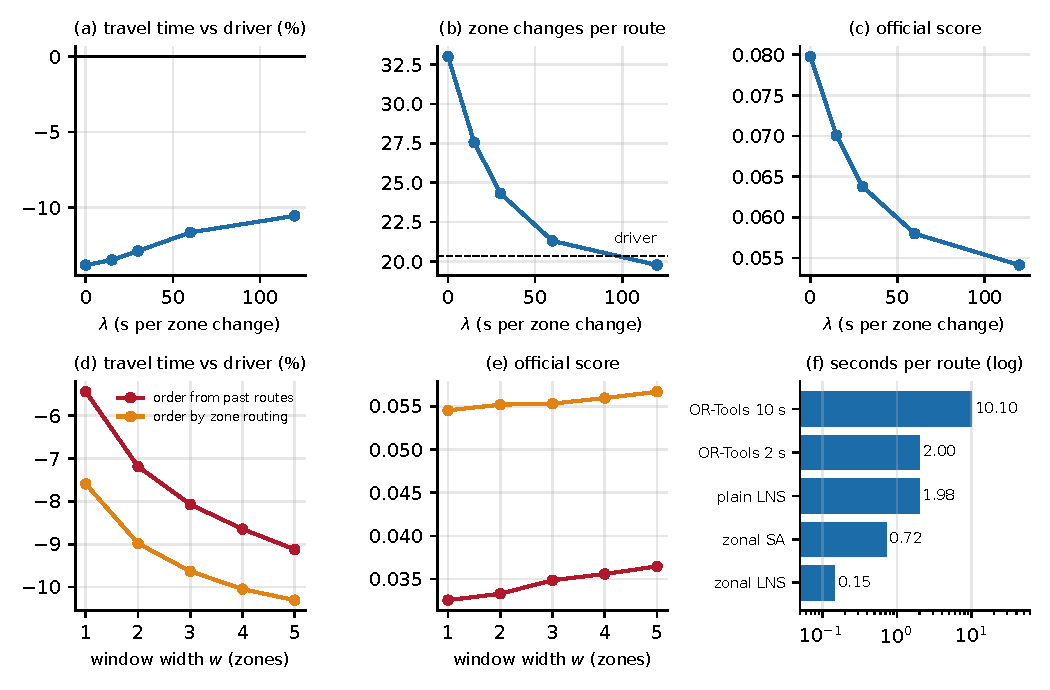
\includegraphics[width=0.95\linewidth]{figures/fig_dev_studies}
\caption{Studies on the development routes. (a) to (c) Plain LNS for increasing zone-change penalty $\lambda$ (seed 0), the dashed line is the zone changes of the real drivers. (d) and (e) Window width $w$ of zonal LNS at $\lambda=60$ s ($w=1$ means no overlap). (f) Mean run time per route (clean run on 20 routes, one process, logarithmic axis).}\label{fig:dev}
\end{figure}

\paragraph{Effect of the penalty $\lambda$ (panels a to c).}\label{sec:lambda}
Each increase of $\lambda$ lowers the number of zone changes and the official score and raises the travel time. The curve flattens. Going from $\lambda=0$ to 30 s removes more than two thirds of the excess zone changes (33.0 to 24.3, against the drivers' 20.3) and costs about 0.9 points of travel time. $\lambda=120$ s reaches the drivers' number of zone changes (19.8) with 10.6\% of travel time saved. This is why we use $\lambda=60$ s as the balanced setting. The official score keeps falling with $\lambda$ but stays above 0.054, because matching the zone \emph{count} does not mean visiting the zones in the driver's order.

\paragraph{Run time (panel f).}\label{sec:time}
Zonal LNS needs about 0.15 s per route for either zone order, roughly 67 times less than OR-Tools at 10 s, and zonal SA needs 0.72 s. Plain LNS takes 2.0 s. OR-Tools uses its whole time limit by design, and a 2 s limit is shown for comparison. The times for the zonal methods do not include the one-off construction of the library of past routes.

\paragraph{Ablation of the zonal pipeline (panels d and e, Table~\ref{tab:ablation}).}\label{sec:ablation}
An \emph{ablation} removes or changes one ingredient of a method and measures how much the result changes. Table~\ref{tab:ablation} does this for zonal LNS with the past-routes order at $\lambda=60$ s. The last two columns give the change against the default (3-zone windows) by paired comparison over routes.
\begin{itemize}
\item \textbf{Overlap helps.} Without overlap (windows of one zone) the saving is $2.62\pm0.25$ points of travel time smaller than with $w=3$. The official score is slightly better without overlap ($-0.0023\pm0.0009$). Wider windows save more time ($w=5$ saves 9.1\%) and give up a little similarity ($0.0365$ against $0.0349$).
\item \textbf{A large neighbourhood helps.} Allowing only up to $m/8$ removed stops inside the windows reduces the saving by $1.56\pm0.19$ points.
\item \textbf{More iterations do not help.} With 500 to 4,500 iterations per window, 300 or 1,000 per zone, or two sweeps, the results differ by 0.1 points or less. The zonal method therefore needs only a small budget.
\end{itemize}

\begin{table}[t]
\centering\small
\caption{Ablation of zonal LNS (past-routes order, $\lambda=60$ s, 207 development routes, seed 0). The last two columns are paired differences to the default. For travel time, positive means less saving than the default, and for the score, negative means closer to the driver.}\label{tab:ablation}
window of 1 zone (no overlap) & $-5.45$ & $0.0326$ & $+2.62\pm0.25$ & $-0.0023\pm0.0009$ \\
window of 2 zones & $-7.19$ & $0.0333$ & $+0.88\pm0.16$ & $-0.0016\pm0.0008$ \\
window of 3 zones (default) & $-8.07$ & $0.0349$ & $+0.00\pm0.00$ & $+0.0000\pm0.0000$ \\
window of 4 zones & $-8.65$ & $0.0356$ & $-0.58\pm0.12$ & $+0.0007\pm0.0006$ \\
window of 5 zones & $-9.12$ & $0.0365$ & $-1.05\pm0.15$ & $+0.0016\pm0.0009$ \\
500 instead of 1,500 iterations per window & $-8.05$ & $0.0347$ & $+0.02\pm0.05$ & $-0.0002\pm0.0004$ \\
4,500 instead of 1,500 iterations per window & $-8.10$ & $0.0349$ & $-0.03\pm0.02$ & $+0.0001\pm0.0001$ \\
300 instead of 1,000 iterations per zone & $-8.07$ & $0.0349$ & $+0.00\pm0.00$ & $+0.0000\pm0.0000$ \\
two sweeps over the windows & $-8.16$ & $0.0348$ & $-0.09\pm0.04$ & $-0.0001\pm0.0002$ \\
small neighbourhood (up to $m/8$ stops removed) & $-6.51$ & $0.0346$ & $+1.56\pm0.19$ & $-0.0003\pm0.0006$ \\
\end{table}

\subsection{How large are the savings?}
Estimated travel time is only a part of the working day. On the development routes it averages 10,923 s, while the service time (time at the doors) averages 16,297 s, so travel time is about 40\% of a route's duration. Service time does not depend on the order. Even the best result, plain LNS, saves about 1,470 s per route on average on these routes, which is 5.4\% of the total route duration of 27,220 s. The estimates also ignore parking, construction and real traffic.

\section{Discussion and limitations}\label{sec:limits}
\paragraph{What the results support.} On this data and with these objectives the following holds.
\begin{enumerate}
\item Plain LNS is the best of the tested methods for estimated travel time. It beats OR-Tools with 10 s per route by a clear margin in under a fifth of the time.
\item A zone-based decomposition makes routes tidier and much faster to compute, but loses travel time compared with plain LNS.
\item The largest gain in similarity to the drivers comes from the zone \emph{order}, and that order has to come from earlier routes of the same depot.
\item Simulated annealing is a sound alternative to LNS inside the zonal pipeline. It gives nearly the same routes and needs more time.
\item The ranking of plain LNS, OR-Tools and the zonal method with the past-routes order is the same at all 17 depots with at least ten routes, and the development routes give results close to the evaluation routes.
\end{enumerate}

\paragraph{What the results do not show.}
\begin{itemize}
\item \textbf{Real driving.} All times are estimates from the data set. We do not know whether a route with less estimated travel time is quicker on the road. The official score is a proxy for driver acceptance and not a measurement of it, and our implementation of it was not compared with Amazon's scorer.
\item \textbf{Constraints we ignore.} Delivery time windows, parcel sizes and service times are not part of the objective. Routes with less travel time might violate time windows that the drivers' routes respect. We therefore do not claim that these routes are feasible in practice.
\item \textbf{Strength of the baseline.} OR-Tools was run with one configuration (guided local search, 10 s), without tuning, and as one time-limited run, in parallel with other processes. A tuned configuration or a longer limit might narrow the gap.
\item \textbf{Not a competition entry.} This report compares general-purpose methods. We did not submit to the challenge and we do not compare our scores with competition results.
\item \textbf{Data.} All results come from one data set, which has two folders from the same source. The past-routes order needs historical routes of the same depot and is not available for a new depot. For the one evaluation route from an unseen depot it falls back to cheapest insertion.
\item \textbf{Tuning.} Settings come from 60 validation routes and several were fixed before a data correction (the missing zone IDs). The zonal settings were not re-tuned. The values $\lambda=0$ and $\lambda=60$ are fixed choices, and $\lambda=60$ was picked after looking at the $\lambda$ study on the development routes. Part of the gap between methods might change with other settings, although the ablation suggests that the iteration budget is not a sensitive choice.
\item \textbf{Statistics.} The intervals in Tables~\ref{tab:paired} and~\ref{tab:ablation} describe variation between routes for one seed. The seed studies use three seeds on the evaluation routes and five on the development routes. They do not cover other data sets.
\end{itemize}

\section{Conclusions}\label{sec:conclusion}
We compared OR-Tools with plain LNS, zonal LNS and zonal SA on the 3,052 evaluation routes of the Amazon Last Mile Routing Challenge. Plain LNS gives the largest saving in estimated travel time (13.9\%, against 11.0\% for OR-Tools) but produces routes that differ from the drivers'. A zone-based pipeline with a zone order taken from earlier routes of the same depot produces routes much closer to the drivers' (official score 0.050 against 0.077 at $\lambda=0$). It saves about five points less travel time (9.1\% against 13.9\%), and on the development routes zonal LNS was about 13 times faster than plain LNS and 67 times faster than OR-Tools per route. The penalty $\lambda$ gives a simple way to move between the two kinds of route. Simulated annealing and LNS perform nearly equally in the zonal pipeline. The next step is a cost model once cost figures are available.

\appendix
\section{Quality check of LNS against exact solvers}\label{app:exact}
To see how close LNS gets to the best possible route, we compared it with the exact solvers of OR-Tools on the first $k$ stops of 15 validation routes for each size $k$ (20 s limit, one worker). Table~\ref{tab:exact} shows the result. CP-SAT (a circuit constraint model) proves optimality for all instances up to 20 stops, but for only 4 of 15 at 40 stops. A textbook mixed-integer formulation (Miller--Tucker--Zemlin constraints, solved with SCIP) is slower at 20 to 30 stops but proves optimality more often at 40 stops (7 of 15). On these small instances LNS found the best known solution in 40 to 67\% of the cases from 15 stops upwards, with a mean excess of at most 0.7\%. On 20 full-size validation routes, CP-SAT (60 s, two workers) warm-started from the LNS route improved it by 0.61\% on average (at most 1.9\%) and proved optimality on 2 of 20. Its proven lower bound is too weak at this size (median gap 24\%) to certify near-optimality. This suggests that plain LNS is within about 1\% of the best possible travel time on a route on average, but it does not prove it.

\begin{table}[h]
\centering\small
\caption{Exact solvers on the first $k$ stops of validation routes (15 instances per size, 20 s limit).}\label{tab:exact}
\begin{tabular}{rR{2.6cm}R{2.6cm}R{3.0cm}R{2.4cm}}
\toprule
$k$ & CP-SAT proved optimal & MIP proved optimal & LNS found best known (\%) & LNS excess (\%) \\
\midrule
10 & 15 & 15 & 100.0 & 0.0 \\
15 & 15 & 15 & 66.7 & 0.4 \\
20 & 15 & 13 & 60.0 & 0.6 \\
25 & 14 & 11 & 40.0 & 0.7 \\
30 & 9 & 9 & 53.3 & 0.5 \\
40 & 4 & 7 & 40.0 & 0.5 \\
\bottomrule
\end{tabular}
\end{table}

\section{Reproducing the results}
All numbers and figures of this report are generated from result files by scripts of the project code, which is not publicly released. The script \texttt{scripts/run\_eval.py} runs the evaluation on the 3,052 routes (our methods for one seed, or OR-Tools with \texttt{--ortools}), \texttt{scripts/run\_final.sh} and \texttt{scripts/run\_seeds.sh} run the experiments on the development routes, and \texttt{paper/make\_paper\_figures.py} and \texttt{paper/make\_eval\_figures.py} write the figures and tables in this document. Method settings are written as specification strings, for example \texttt{lns:i=5000:kmax=2:l=60} (plain LNS, 5,000 iterations, $\lambda=60$) or \texttt{zlns:order=ref:w=3:ii=1000:wi=1500:kmax=2:l=60} (zonal LNS with the past-routes order).

\bibliography{references}

\end{document}
